\pdfminorversion=7
\documentclass[spanish,aspectratio=1610,xcolor={dvipsnames,table}]{beamer}
\geometry{paperwidth=19.2cm,paperheight=12cm}

\usepackage[utf8]{inputenc}
\usepackage[T1]{fontenc}
\usepackage[spanish,es-nodecimaldot]{babel}
\usepackage{lmodern,amsmath,amssymb,booktabs,array,graphicx,ragged2e,tikz,hyperref}
\usetikzlibrary{arrows.meta,positioning,calc,fit,backgrounds}

\newcommand{\studentname}{Mtro. Martín Jonathan de la Cruz Muñoz}
\newcommand{\studentshort}{M. de la Cruz Munoz}
\newcommand{\studentid}{00874}
\newcommand{\studentemail}{martin.delacruz@campus.iiiepe.edu.mx}
\newcommand{\programname}{Maestría en Enseñanza y Aprendizaje de las Matemáticas}
\newcommand{\programshort}{MAEM}
\newcommand{\coursecode}{PFM02}
\newcommand{\coursename}{Temas selectos de matemáticas I}
\newcommand{\courseperiod}{Ago--Nov 2026 (SD26)}
\newcommand{\institutionname}{IIIEPE}
\newcommand{\iiiepelogo}{img/iiiepe/logo-iiiepe-blanco.png}
\newcommand{\iiiepemark}{img/iiiepe/marca-iiiepe.png}

\definecolor{iiiepeNavy}{HTML}{163B5C}
\definecolor{iiiepeBlue}{HTML}{1F6F9F}
\definecolor{iiiepeAqua}{HTML}{20B7A8}
\definecolor{iiiepeOrange}{HTML}{F28C28}
\definecolor{iiiepePaper}{HTML}{F6F8F7}
\definecolor{iiiepeInk}{HTML}{1E2A32}

\mode<presentation>{
  \usetheme{default}
  \usefonttheme{professionalfonts}
  \setbeamertemplate{navigation symbols}{}
  \setbeamertemplate{blocks}[rounded][shadow=false]
}
\hypersetup{colorlinks=true,urlcolor=iiiepeBlue,linkcolor=iiiepeNavy}
\setbeamercolor{background canvas}{bg=white}
\setbeamercolor{normal text}{fg=iiiepeInk,bg=white}
\setbeamercolor{structure}{fg=iiiepeBlue}
\setbeamercolor{frametitle}{fg=white,bg=iiiepeNavy}
\setbeamercolor{title}{fg=white,bg=iiiepeNavy}
\setbeamercolor{block title}{fg=white,bg=iiiepeBlue}
\setbeamercolor{block body}{fg=iiiepeInk,bg=iiiepePaper}
\setbeamercolor{block title alerted}{fg=white,bg=iiiepeOrange}
\setbeamercolor{block body alerted}{fg=iiiepeInk,bg=iiiepeOrange!10}
\setbeamerfont{title}{size=\Large,series=\bfseries}
\setbeamerfont{frametitle}{size=\fontsize{13}{17}\selectfont,series=\bfseries}
\setbeamerfont{block title}{series=\bfseries}
\setbeamertemplate{itemize item}{\textcolor{iiiepeAqua}{$\blacktriangleright$}}

\newcommand{\localLogo}[1]{\IfFileExists{#1}{\includegraphics[height=0.55cm]{#1}}{\textbf{\institutionname}}}
\setbeamertemplate{frametitle}{
  \nointerlineskip
  \begin{beamercolorbox}[wd=\textwidth,ht=1.0cm,dp=0.2cm,leftskip=0.35cm,rightskip=0.25cm]{frametitle}
    \begin{minipage}[c]{0.72\textwidth}\insertframetitle\end{minipage}\hfill\raisebox{-0.08cm}{\localLogo{\iiiepelogo}}
  \end{beamercolorbox}
  \vspace{-0.04cm}{\color{iiiepeOrange}\rule{\textwidth}{1.3pt}}
}
\setbeamertemplate{footline}{
  \leavevmode\hbox{%
    \begin{beamercolorbox}[wd=.34\paperwidth,ht=2.7ex,dp=1ex,leftskip=1em]{author in head/foot}\color{white}\studentshort\end{beamercolorbox}%
    \begin{beamercolorbox}[wd=.42\paperwidth,ht=2.7ex,dp=1ex,center]{title in head/foot}\color{white}\programshort\ -- \coursecode\ (SD26)\end{beamercolorbox}%
    \begin{beamercolorbox}[wd=.24\paperwidth,ht=2.7ex,dp=1ex,rightskip=1em plus 1fil]{date in head/foot}\color{white}Matrícula \studentid\hfill\insertframenumber/\inserttotalframenumber\end{beamercolorbox}%
  }
}
\setbeamercolor{author in head/foot}{bg=iiiepeNavy}
\setbeamercolor{title in head/foot}{bg=iiiepeBlue}
\setbeamercolor{date in head/foot}{bg=iiiepeNavy}

\title{El lugar perfecto}
\subtitle{Actividad 2 (Sesión 9) · Mediatrices, Bisectrices, Circuncentro e Incentro en GeoGebra}
\author{\studentname\ (Matrícula \studentid)}
\institute{\institutionname\ · \programname}
\date{17 de octubre de 2026}

\begin{document}
\begin{frame}[plain]
  \centering
  \vspace{0.5cm}
  \IfFileExists{\iiiepemark}{\includegraphics[height=1.6cm]{\iiiepemark}}{}
  \vspace{0.35cm}
  \begin{beamercolorbox}[sep=10pt,center,rounded=true,wd=0.88\textwidth]{title}
    {\Large\bfseries El lugar perfecto}\\[6pt]
    {\small\color{iiiepePaper} Actividad 2 (Sesión 9) · Mediatrices, Bisectrices, Circuncentro e Incentro en GeoGebra}
  \end{beamercolorbox}
  \vspace{0.45cm}
  {\normalsize\bfseries \studentname}\\
  {\small Matrícula \studentid\ · \coursename\ (\coursecode) · \courseperiod}\\
  {\footnotesize 17 de octubre de 2026}
\end{frame}

\begin{frame}{Retos de Equidistancia: Mediatriz y Bisectriz}
  \begin{columns}[T]
    \column{0.48\textwidth}
      \begin{block}{Mediatriz y Circuncentro ($O$)}
        \begin{itemize}
          \item Equidista de dos vértices $A$ y $B$ (bebedero).
          \item Para tres salones no colineales $A,B,C$, dos mediatrices determinan $O$ con $OA = OB = OC$.
          \item Centro de la circunferencia circunscrita.
        \end{itemize}
      \end{block}
    \column{0.48\textwidth}
      \begin{block}{Bisectriz e Incentro ($I$)}
        \begin{itemize}
          \item Equidista perpendicularmente de dos rectas concurrentes (caminos).
          \item Las tres bisectrices interiores concurren en $I$.
          \item Centro de la circunferencia inscrita (siempre interior).
        \end{itemize}
      \end{block}
  \end{columns}
\end{frame}

\begin{frame}{Evidencia GeoGebra: Equidistancia y Tipos de Triángulo}
  \begin{columns}[T]
    \column{0.49\textwidth}
      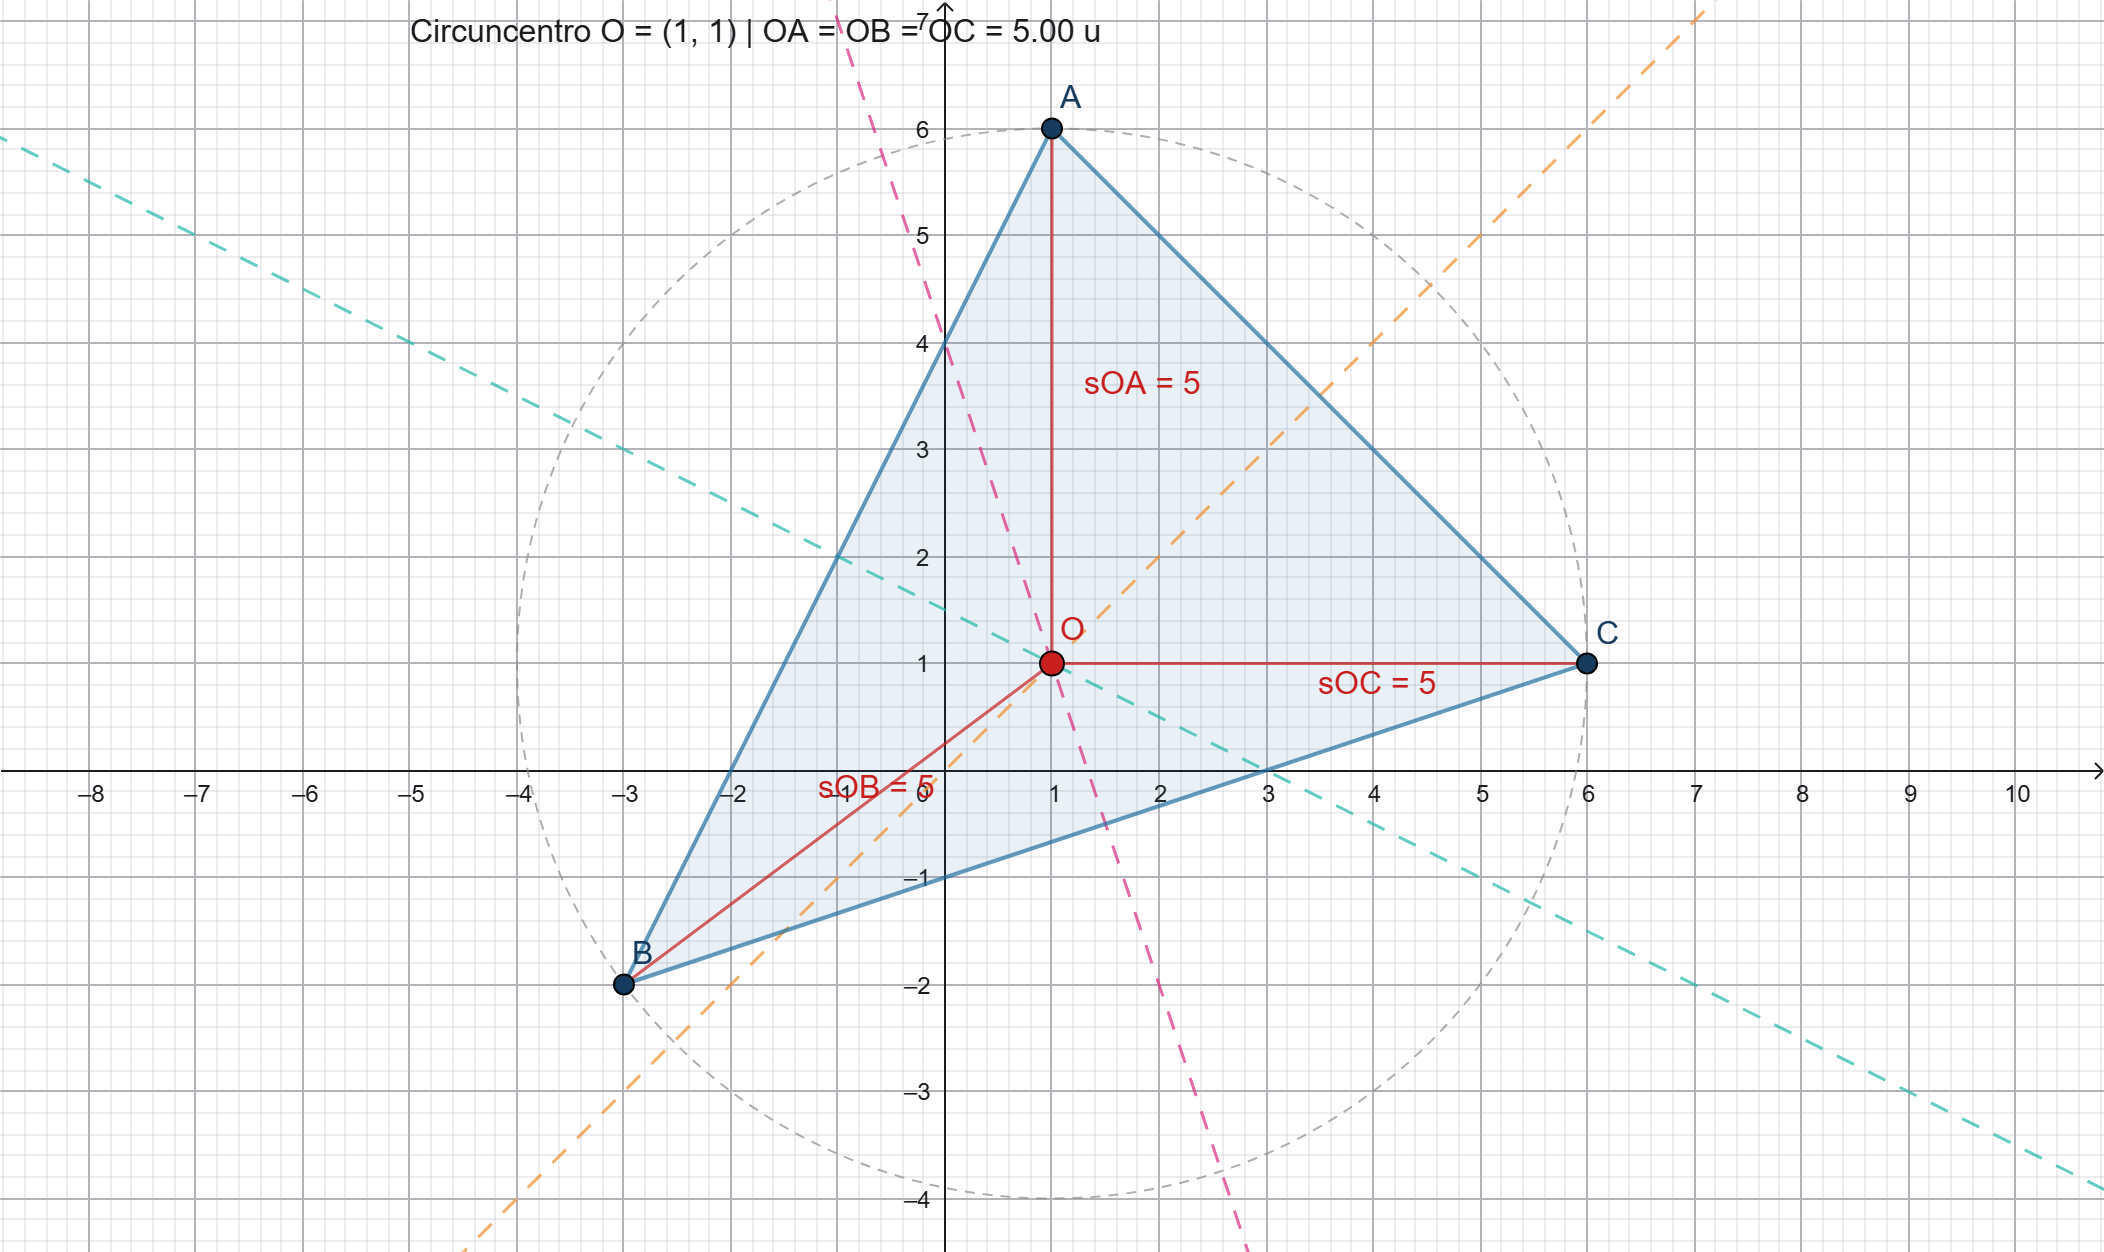
\includegraphics[width=\linewidth]{img/geogebra/act2_a_mediatrices_equidistancia.png}
      {\scriptsize Actividad a: $O=(1,1)$, $OA=OB=OC=5\text{ u}$.}
    \column{0.49\textwidth}
      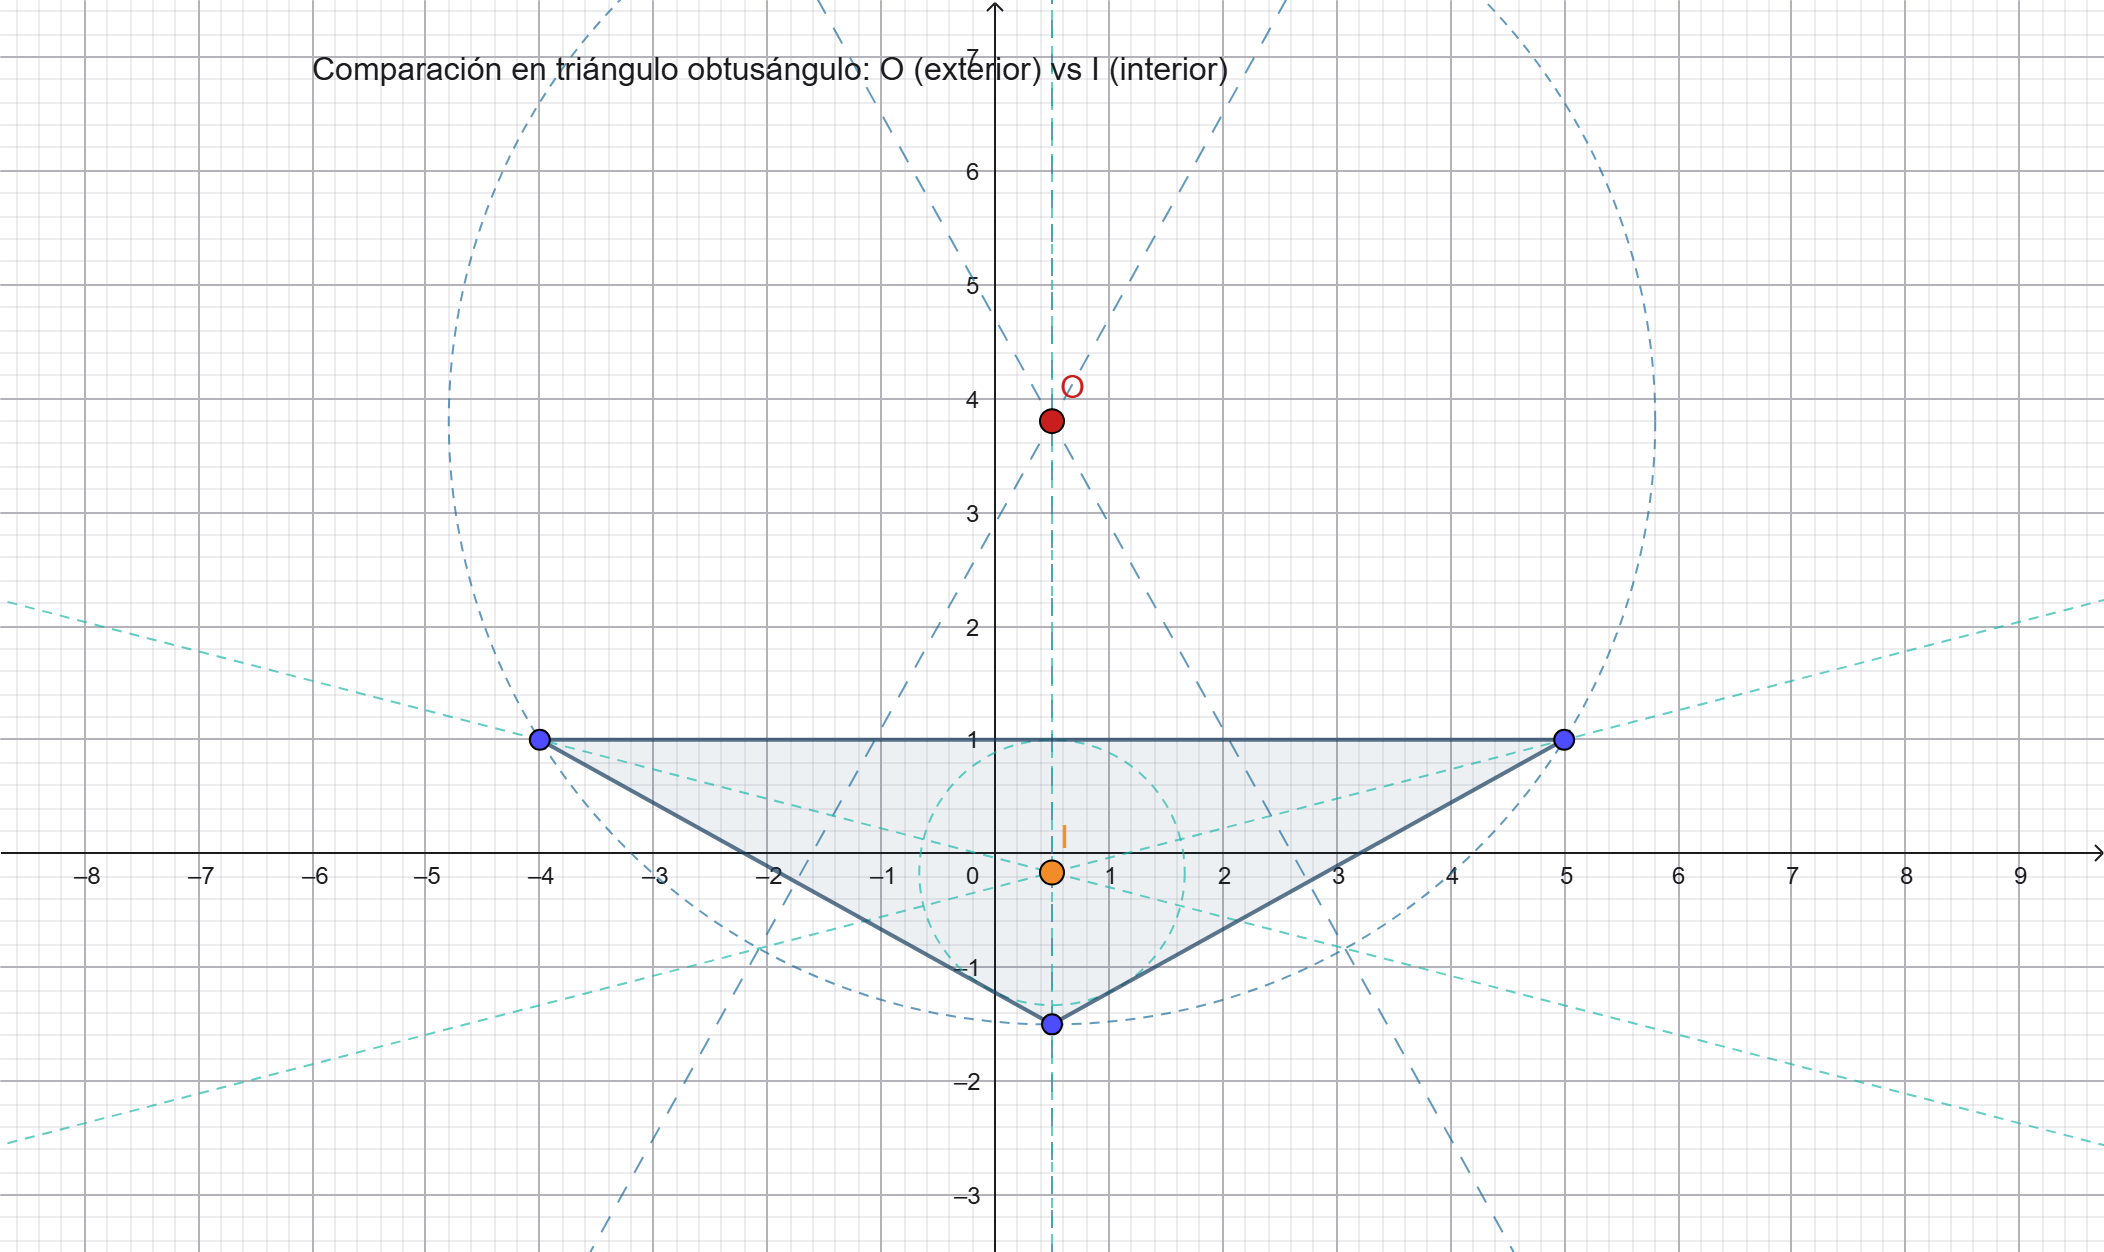
\includegraphics[width=\linewidth]{img/geogebra/act2_d_comparacion_circuncentro_incentro.png}
      {\scriptsize Actividad d: $O$ exterior vs. $I$ interior en obtusángulo.}
  \end{columns}
\end{frame}

\begin{frame}{Síntesis Comparativa y Reflexión Didáctica}
  \begin{center}
  \small
  \begin{tabular}{lll}
    \toprule
    \textbf{Triángulo} & \textbf{Ubicación de $O$} & \textbf{Ubicación de $I$} \\
    \midrule
    Acutángulo  & Interior & Interior \\
    Rectángulo  & Punto medio de la hipotenusa & Interior \\
    Obtusángulo & Exterior & Interior \\
    \bottomrule
  \end{tabular}
  \end{center}
  \vspace{0.2cm}
  \begin{block}{Mediación docente en secundaria}
    \begin{itemize}
      \item Formalizar los términos \textit{circuncentro} e \textit{incentro} \textbf{después} de la experimentación con regla, compás y GeoGebra.
      \item Prevenir la confusión entre mediatriz y mediana exigiendo verificar perpendicularidad y punto medio.
    \end{itemize}
  \end{block}
\end{frame}

\end{document}
